\subsection{Turing Test}
In addition to the aforementioned quantitative metrics, we decided to perform a short Turing test, to use also
a qualitative metric in the models comparison. To do so, we created a short survey on Google Forms. The survey is
made of two parts: in the first part we show the participants three different black and white images, each one of
them followed by the corresponding colorized images; while for the second part we chose 4 different images, which
are originally colored, and we displayed the corresponding colorized images, without showing the original image.
For all the automatically colorized images, we asked the participant to say how realist the colorization was in a
scale that goes from 1 (not realistic at all) to 5 (very realistic). Note that for the Turing Test we employed only images coming from the four best
performing models, i.e. Eccv16, Siggraph17, ChromaGAN and InstColorization.

We collected answers from 124 different subjects and in Figure \ref{fig:turing} we can see the mean scores
obtained by the differnt models. From the plots we can clearly see that the models performed differently on black and white images and on colored
images. This can be explained by the fact that black and white pictures and colored pictures are taken using
different technologies.
However, the models that obtained the higest scores in both cases are Siggraph17 and ChromaGAN.

\begin{figure}[h]
	\centering
	\captionsetup[subfigure]{labelformat=empty}
	\begin{subfigure}[b]{0.1\textwidth}
		\begin{adjustwidth}{-1.1cm}{}
		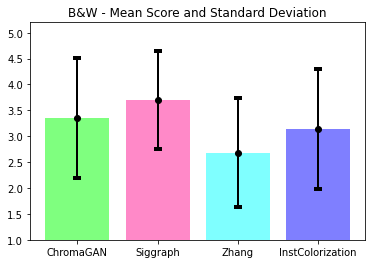
\includegraphics[width=4cm]{bw turing.png}
		\end{adjustwidth}
	\caption{B\&W}
	\end{subfigure}
\hspace{2.3cm}
	\begin{subfigure}[b]{0.1\textwidth}
		\begin{adjustwidth}{-1.1cm}{}
			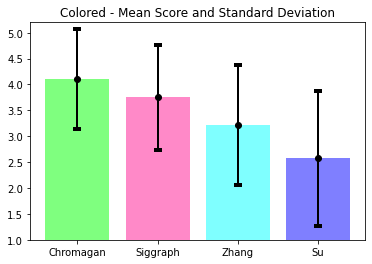
\includegraphics[width=4cm]{col turing.png}
		\end{adjustwidth}
		\caption{Colored}
	\end{subfigure}
	\caption{{\small Mean scores obtained with the colorization on black and white photographs and originally colored images.}}
	\label{fig:turing}
\end{figure}